\documentclass[DIV=calc, paper=a4, fontsize=11pt]{scrartcl}


\usepackage{makeidx}
\usepackage{graphicx}
\usepackage{flushend}

\usepackage{lmodern}
\usepackage[left=1.5cm,right=1.5cm,top=2.5cm,bottom=2cm]{geometry}
\usepackage{float}		
\bibliographystyle{plain} 
\pagestyle{plain} 
\pagenumbering{arabic}
\usepackage{fancyhdr} 	


\usepackage[T1]{fontenc}
\usepackage[utf8]{inputenc}
\usepackage[spanish]{babel}
\usepackage{hyperref}
\usepackage{graphicx}

\usepackage{lipsum}
\usepackage[protrusion=true,expansion=true]{microtype}
\usepackage{amsmath,amsfonts,amsthm}
\usepackage[svgnames]{xcolor}
\usepackage[svgnames]{xcolor}
\usepackage{booktabs}
\usepackage{fix-cm}
\usepackage{multicol}
\usepackage{siunitx}
\newenvironment{Figura}
  {\par\medskip\noindent\minipage{\linewidth}}
  {\endminipage\par\medskip}

\usepackage{sectsty}
\allsectionsfont{\usefont{OT1}{phv}{b}{n}}

\usepackage{fancyhdr}
\pagestyle{fancy}
\usepackage{lastpage}

\lhead{}
\chead{}
\rhead{}

\lfoot{}
\cfoot{}
\rfoot{\footnotesize Page \thepage\ of \pageref{LastPage}}

\renewcommand{\headrulewidth}{0.0pt}
\renewcommand{\footrulewidth}{0.4pt}

\usepackage{lettrine}
\newcommand{\initial}[1]{\lettrine[lines=3,lhang=0.3,nindent=0em]{
\color{DarkGoldenrod}{\textsf{#1}}}{}}

\usepackage{titling}

\newcommand{\HorRule}{\color{DarkGoldenrod} \rule{\linewidth}{1pt}}

\pretitle{\vspace{-120pt} \begin{flushleft} \HorRule \fontsize{22}{35} \usefont{OT1}{phv}{b}{n} \color{DarkRed} \selectfont}

\title{Circuitos eléctricos de C.D.\\ %Aquí va el nombre de la práctica 
Práctica 1}

\posttitle{\par\end{flushleft}\vskip 0.5em}

\preauthor{\begin{flushleft}\large \lineskip 0.5em \usefont{OT1}{phv}{b}{sl} \color{DarkRed}}

\author{García Perez Angel Yair\\
Macías Márquez Misael Iván \\
Martínez Morales Isaac David }

\postauthor{\footnotesize \usefont{OT1}{phv}{m}{sl} \color{Black}

\vspace*{0.1cm} Facultad de Ciencias, UNAM

\par\end{flushleft}\HorRule}

\date{Jueves 10 de Marzo de 2022\\Semestre 2022-1}


\begin{document}

\maketitle


\begin{abstract}
 
\textbf{Resumen:} 
En esta practica, a través de un simulador, se intentó probar experimentalmente el principio de superposición en un circuito para una resistencia de $1k\Omega $, no se logró probar porque las incertidumbres estaban subestimadas, además se midieron todos los voltajes y todas las corrientes del circuito, también se aplicó el Teorema de Thévenin para medir resistencias y voltajes equivalentes, se obtuvo que $R_{eq}=(733.590\pm0.082) \Omega$, $V_{eq}=(10.83529\pm1.0888\times10^{-3})V$, el Teorema de Norton se aplicó para medir resistencias e intensidades equivalentes, se obtuvo $R'_{eq}=(733.426\pm0.082) \Omega$ y $I'_{eq}=(14.60056\pm 0.01230)m A$, también se comprobó que $V_{eq}=I'_{eq}R'_{eq}$ y que $R_{eq}=R'_{eq}$.

\end{abstract}

\begin{multicols}{2}




\section*{Introducción}
El propósito de esta practica fue tomar datos, para así familiarizarse con el equipo de laboratorio, también el propósito fue poner en practica los conocimientos adquiridos para la toma de incertidumbres.
\subsection*{Objetivos}

\begin{enumerate}
    \item Comprobar el principio de superposición solo en $\mathbf{R6}$.
    
    \item Medir el voltaje de cada elemento del circuito.
    
    \item Medir la corriente de cada elemento del circuito.
    
    \item Aplicando el teorema de Thévenin, medir en $\mathbf{R6}$ la resistencia y voltaje equivalente.
    
    \item Aplicando el teorema de Norton, medir en $\mathbf{R6}$ la resistencia y corriente equivalente.
    
    
\end{enumerate}


\subsection*{Principio de Superposición}

En cualquier red resistiva lineal, la tensión o la corriente a través de cualquier resistencia o
fuente se calcula mediante la suma algebraica de todas las tensiones o corrientes individuales ocasionadas por fuentes independientes separadas que actúan solas, junto con todas las demás
fuentes de tensión independientes sustituidas por cortocircuitos y todas las demás fuentes de
corriente independientes, sustituidas por circuitos abiertos[1].


\subsection*{Teorema de Thévenin}

El Teorema de Thévenin recibe su nombre en honor a L. C. Thévenin, ingeniero francés quien trabajaba en telegrafía y que publicó el teorema en 1883, el enunciado del teorema es el siguiente[1]:

\begin{itemize}
    \item Dado cualquier circuito lineal, arreglarlo nuevamente en la forma de dos
redes A y B conectadas por dos alambres. A es la red que se simplificará; B
se dejará intacta.

\item Desconectar la red B. Definir una tensión $v_{oc}$ como la tensión que ahora
aparece en las terminales de la red A.

\item Apagar o “asignar cero a” toda fuente independiente de la red A para
formar una red inactiva. Dejar las fuentes dependientes intactas.

\item Conectar una fuente de tensión independiente con un valor de $v_{oc}$ en
serie con la red inactiva. No terminar el circuito; dejar desconectadas las
dos terminales.

\item  Conectar la red B a las terminales de la nueva red A. Todas las corrientes
y tensiones de B permanecerán intactas.
\end{itemize} 




\subsection*{Teorema de Norton}

El teorema de Norton recibe su nombre en honor a E. L. Norton, científico de los Bell Telephone Laboratories, ekl enunciado del teorema es el siguiente[1]:

\begin{itemize}
    \item Dado cualquier circuito lineal, volver a ordenar en la forma de dos
redes A y B conectadas por dos alambres. La red que se va a simplificar
es A; B se dejará intacta. Como se hizo antes, si cualquiera de las redes
contiene una fuente dependiente, su variable de control debe estar en la
misma red.

\item Desconectar la red B y poner en cortocircuito las terminales de A. Definir una corriente isc como la corriente que circula ahora a través de las terminales cortocircuitadas de la red A.

\item Apagar o “asignar cero” a todas las fuentes independientes de la red
A para formar una red inactiva. Dejar las fuentes dependientes intactas.

\item Conectar una fuente de corriente independiente de valor $i_{sc}$ en paralelo
con la red inactiva. Dejar el circuito sin terminar; dejar desconectadas las
dos terminales.

\item Conectar la red B a las terminales de la nueva red A. Todas las corrientes y tensiones en B permanecerán intactas.


\end{itemize}



\section*{Metodología}

En el simulador Multisim se utilizaron multímetros Agilent 34401A de $6^{1/2}$ dígitos, 6 resistencias de distintos valores con una tolerancia del $5\%$, 2 fuentes de poder una de voltaje y otra de corriente con un $2\%$ de tolerancia y una tierra física.

\begin{Figura}
    \centering
    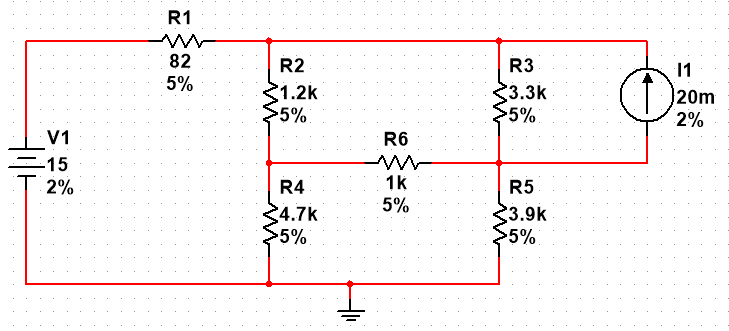
\includegraphics[width=1\textwidth]{circuito.PNG}
    \captionof{figure}{Arreglo experimental: simulación en Multisim, $\mathbf{R1}$ - $\mathbf{R6}$ resistencias de 1/2 W, \mathbf{V1} fuente de voltaje, $\mathbf{I1}$ fuente de corriente, $\mathbf{XMMi}$ multímetro i-ésimo.}
    \label{fig}
\end{Figura}

\subsection*{Objetivo 1}

Para comprobar el principio de superposición en la resistencia $\mathbf{R6}$ se desconectó la fuente de corriente $\mathbf{I1}$ y con el multímetro $\mathbf{XMM1}$ configurado como voltímetro se midió el voltaje en la resistencia $\mathbf{R6}$ (ver figura 2).

Ahora con la fuente de corriente $\mathbf{I1}$ conectada y la fuente de voltaje $\mathbf{V1}$ cortocircuitada y desconectada, se midió nuevamente el voltaje en $\mathbf{R6}$ con ayuda del multímetro $\mathbf{XMM1}$ (ver en la figura 3).

Por ultimo, se repitió la medición del voltaje en $\mathbf{R6}$ pero con el circuito original, es decir, sin desconectar ni cortocircuitar ninguna fuente de poder (ver figura 4).

\subsection*{Objetivo 2}

Con la finalidad de medir el voltaje en cada elemento del circuito original , se conectaron en paralelo multímetros $\mathbf{XMM1}-\mathbf{XMM8}$ configurados como voltímetros en cada elemento (ver figura 5). 

\subsection*{Objetivo 3}

A fin de medir la corriente en cada elemento del circuito original , se conectaron en serie multímetros $\mathbf{XMM1}-\mathbf{XMM8}$ configurados como amperímetros en cada elemento (ver figura 6).

\subsection*{Objetivo 4}

Para aplicar el teorema de Thévenin primero con el multímetro $\mathbf{XMM1}$ en paralelo configurado como voltímetro, se midió el voltaje en la resistencia $\mathbf{R6}$ (ver figura 7).

Después con el mismo multímetro en paralelo pero configurado como ohmetro se midió la resistencia equivalente en $\mathbf{R6}$ con la fuente de voltaje $\mathbf{V1}$ cortocircuitada y desconectada, también se desconectó la fuente de corriente $\mathbf{I1}$ (ver figura 8).


\subsection*{Objetivo 5}

Para aplicar el teorema de Norton se utilizó el multímetro $\mathbf{XMM1}$ en paralelo configurado como amperímetro para medir la corriente en $\mathbf{R6}$  en el circuito original (ver figura 9).

Por último de forma análoga al objetivo 4, con el multímetro configurado igual y en paralelo se midió la resistencia equivalente en $\mathbf{R6}$ 




\section*{Simulación\footnote{Las unidades en algunas figuras no se muestran aunque se pueden inferir fácilmente por el diagrama de cada elemento.}}

\subsection*{Objetivo 1}

\begin{Figura}
    \centering
    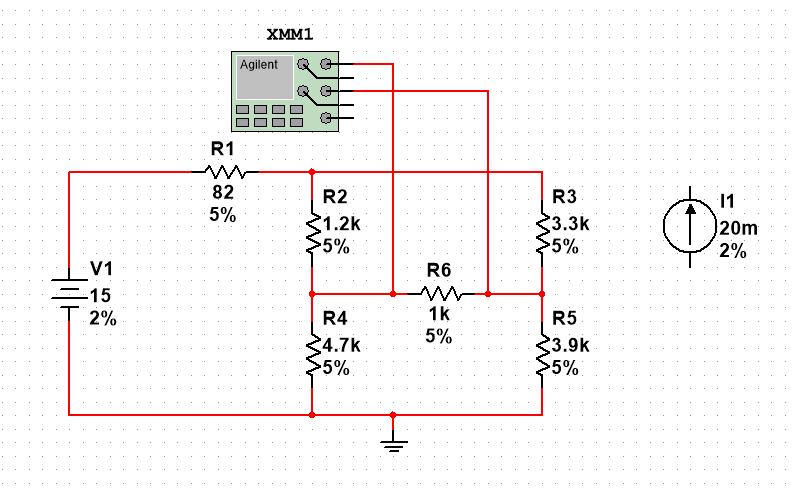
\includegraphics[width=1\textwidth]{1,a.PNG}
    \captionof{figure}{Comprobación del principio de superposición para $\mathbf{R6}$: medición del voltaje en $\mathbf{R6}$ con la fuente de corriente desconectada.}
    \label{fig}
\end{Figura}

\begin{Figura}
    \centering
    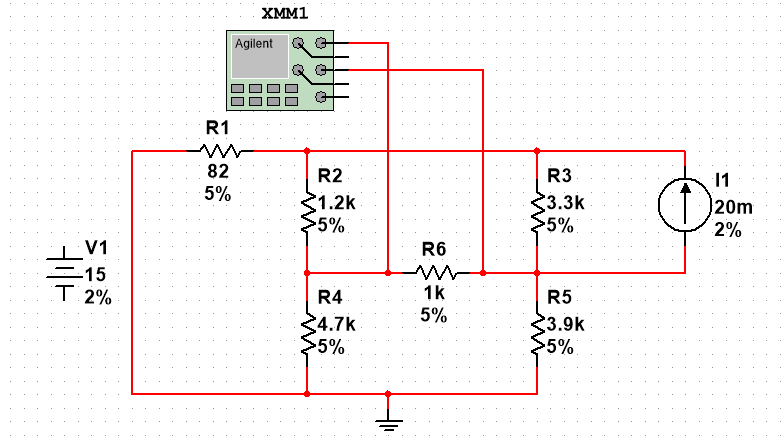
\includegraphics[width=1\textwidth]{1.b.PNG}
    \captionof{figure}{Comprobación del principio de superposición para $\mathbf{R6}$: medición del voltaje en $\mathbf{R6}$ con la fuente de voltaje cortocircuitada y desconectada.}
    \label{fig}
\end{Figura}

\begin{Figura}
    \centering
    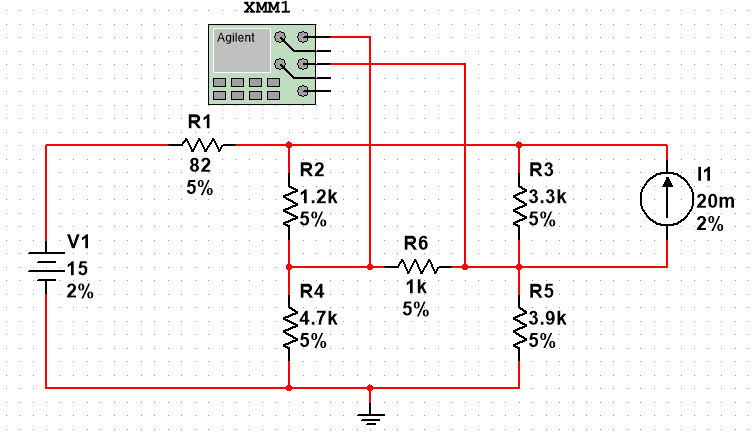
\includegraphics[width=1\textwidth]{1.completo.PNG}
    \captionof{figure}{Comprobación del principio de superposición para $\mathbf{R6}$: medición del voltaje en $\mathbf{R6}$ con el circuito original.}
    \label{fig}
\end{Figura}

\subsection*{Objetivo 2}


\begin{Figura}
    \centering
    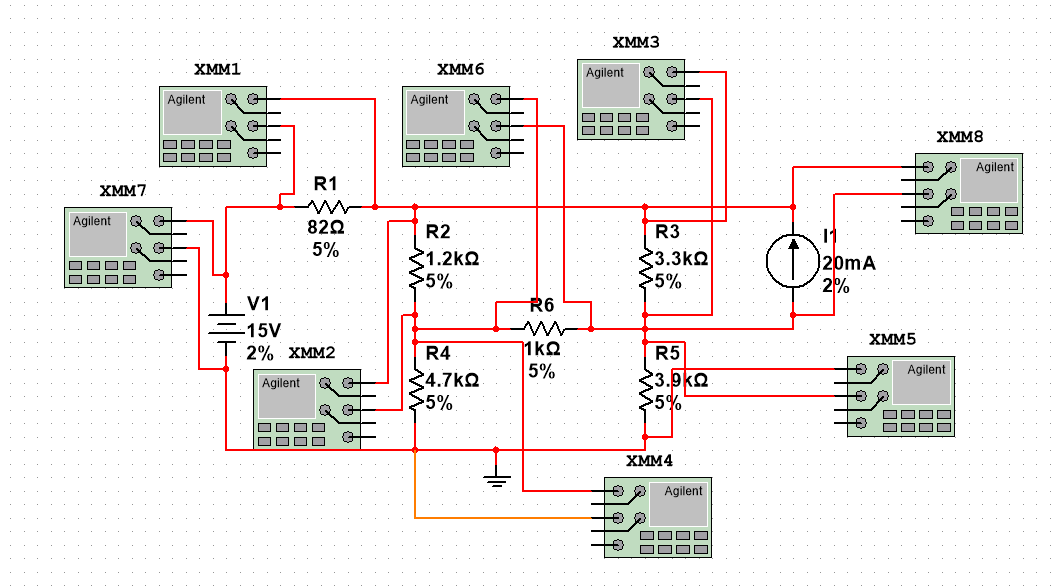
\includegraphics[width=1\textwidth]{circuito voltajes.PNG}
    \captionof{figure}{Medición de voltajes: multímetros $\mathbf{XMM1}-\mathbf{XMM8}$ conectados en paralelo para cada elemento del circuito original.}
    \label{fig}
\end{Figura}

\subsection*{Objetivo 3}

\begin{Figura}
    \centering
    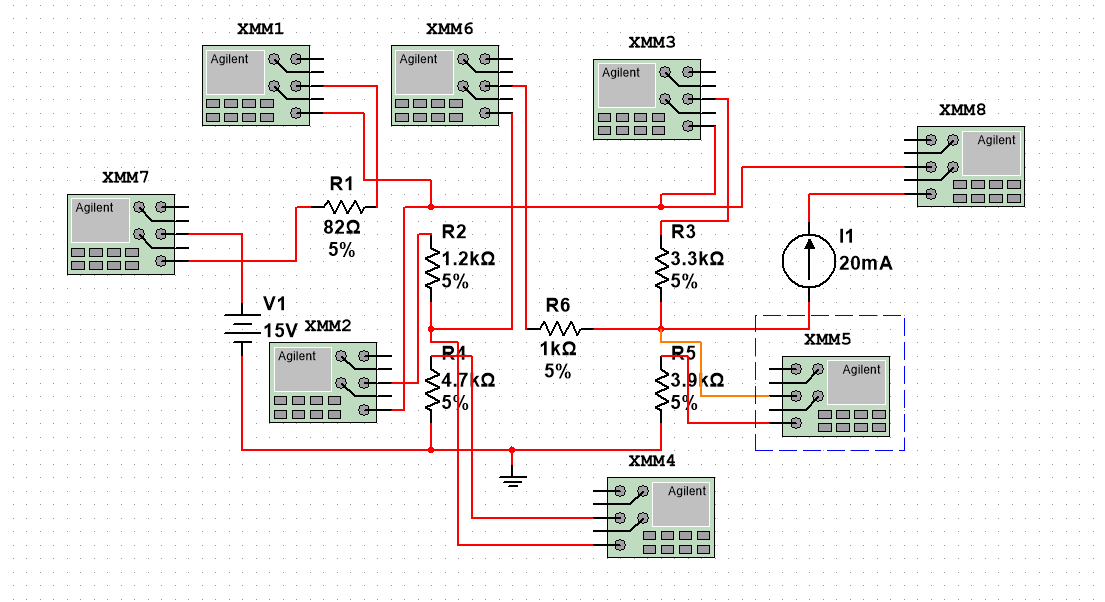
\includegraphics[width=1\textwidth]{circuito corrientes.PNG}
    \captionof{figure}{Medición de corrientes: multímetros $\mathbf{XMM1}-\mathbf{XMM8}$ conectados en paralelo para cada elemento del circuito original.}
    \label{fig}
\end{Figura}

\subsection*{Objetivo 4}

\begin{Figura}
    \centering
    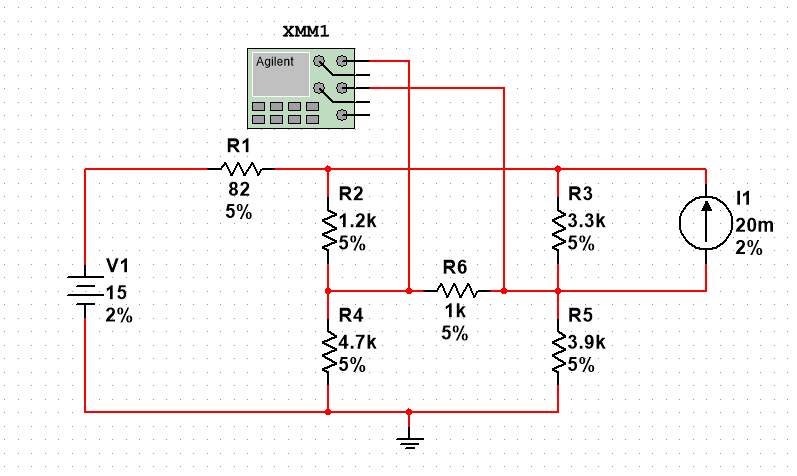
\includegraphics[width=1\textwidth]{T1.PNG}
    \captionof{figure}{Aplicación del teorema de Thévenin en $\mathbf{R6}$: medición del voltaje en $\mathbf{R6}$ con el circuito original. }
    \label{fig}
\end{Figura}

\begin{Figura}
    \centering
    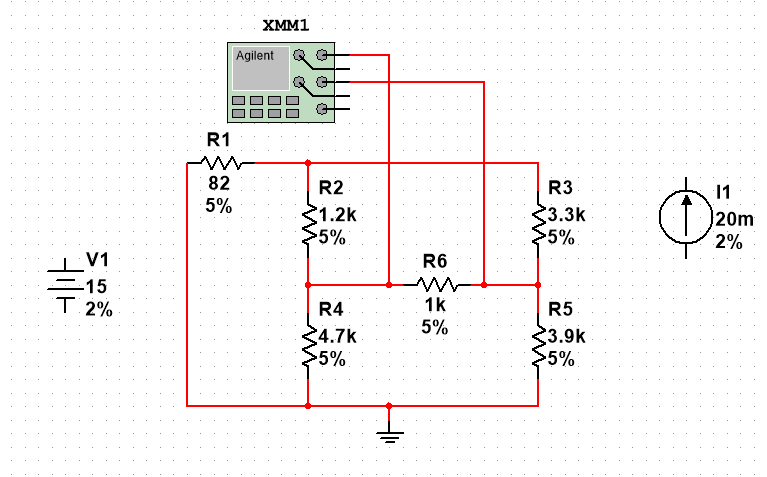
\includegraphics[width=1\textwidth]{T2.PNG}
    \captionof{figure}{Aplicación del teorema de Thévenin en $\mathbf{R6}$: medición de la resistencia en $\mathbf{R6}$ con la fuente de corriente desconectada y la fuente de voltaje cortocircuitada y desconectada. }
    \label{fig}
\end{Figura}

\subsection*{Objetivo 5}

\begin{Figura}
    \centering
    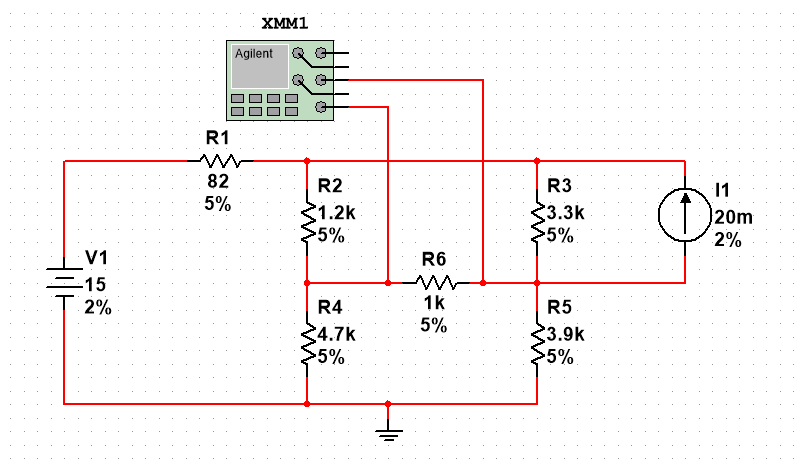
\includegraphics[width=1\textwidth]{N1.PNG}
    \captionof{figure}{Aplicación del teorema de Norton en $\mathbf{R6}$: medición de la corriente en $\mathbf{R6}$ con el circuito original.}
    \label{fig}
\end{Figura}


\begin{Figura}
    \centering
    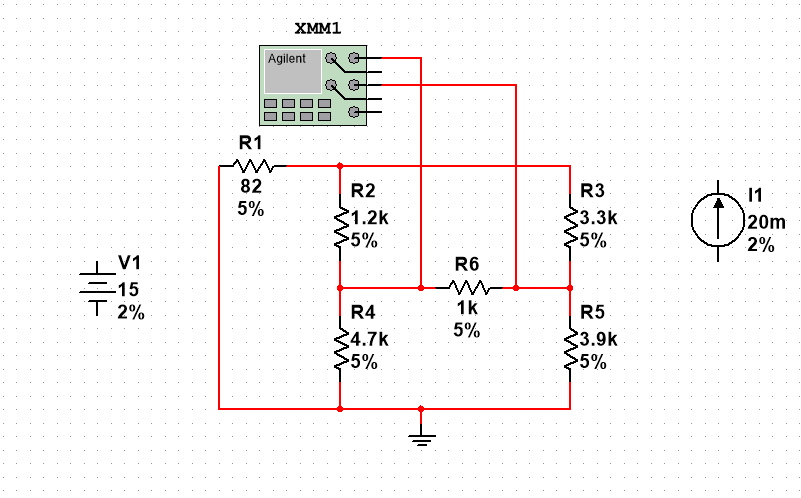
\includegraphics[width=1\textwidth]{N2.PNG}
    \captionof{figure}{Aplicación del teorema de Norton en $\mathbf{R6}$: medición de la resistencia en $\mathbf{R6}$ con la fuente de corriente desconectada y la fuente de voltaje cortocircuitada y desconectada.}
    \label{fig}
\end{Figura}





\section*{Resultados y Observaciones}

\subsection*{Objetivo 1}

Los voltajes medidos con sus incertidumbres (ver anexos) son:

\begin{equation*}
    V_1 = (1.056413 \pm 0.008697) V 
\end{equation*}

\begin{equation*}
    V_2 = (9.51713 \pm 0.03830) V
\end{equation*}

\begin{equation*}
    V_3 = (10.83529 \pm 0.10876) V
\end{equation*}

\noindent para las figuras 2, 3 y 4 respectivamente. 



\subsection*{Objetivo 2}

Los voltajes medidos con sus incertidumbres (ver anexos) son:

\begin{equation*}
    V_1 = (138.9636 \pm 0.0104) V
\end{equation*}

\begin{equation*}
    V_2 = (13.30603 \pm \num{5.157e-4}) V
\end{equation*}

\begin{equation*}
    V_3 = (23.5114 \pm \num{1.658e-3}) V
\end{equation*}

\begin{equation*}
    V_4 = (1.834834 \pm \num{1.142e-4}) V
\end{equation*}

\begin{equation*}
    V_5 = (8.37054 \pm \num{3.430e-4}) V
\end{equation*}

\begin{equation*}
    V_6 = (10.20537 \pm \num{1.059 e -3}) V
\end{equation*}

\begin{equation*}
    V_7 = (15.00190 \pm \num{1.275e-3}) V
\end{equation*}

\begin{equation*}
    V_8 = (23.5114 \pm \num{1.658e-3}) V
\end{equation*}




\noindent para la figura 5. 


\subsection*{Objetivo 3}


Las corrientes medidas con sus incertidumbres (ver anexos) son:

\begin{equation*}
    I_1 = (1.891151 \pm \num{2.946e-3}) mA
\end{equation*}

\begin{equation*}
    I_2 = (10.86479 \pm 0.01043) mA
\end{equation*}

\begin{equation*}
    I_3 = (7.24405 \pm \num{5.622e-3}) mA
\end{equation*}

\begin{equation*}
    I_4 = (0.286872 \pm \num{2.193e-3}) mA 
\end{equation*}

\begin{equation*}
    I_5 = (2.27802 \pm \num{3.139e-3}) mA
\end{equation*}

\begin{equation*}
    I_6 = (10.47792 \pm 0.01024) mA
\end{equation*}

\begin{equation*}
    I_7 = (1.891151 \pm \num{2.946e-3}) mA
\end{equation*}

\begin{equation*}
    I_8 = (20 \pm 0.015) mA
\end{equation*}




\noindent para la figura 6. 

\subsection*{Objetivo 4}

El voltaje medido con su incertidumbre (ver anexos) es:

\begin{equation*}
    V = (10.83529 \pm \num{1.0888e-3} ) V
\end{equation*}

\noindent para la figura 7.

La resistencia medida con su incertidumbre (ver anexos) es:

\begin{equation*}
    R = (733.590 \pm 0.082) \Omega
\end{equation*}

\noindent para la figura 8.


\subsection*{Objetivo 5}


La corriente medida con su incertidumbre (ver anexos) es:

\begin{equation*}
    I = (14.60056 \pm 0.01230) mA
\end{equation*}

\noindent para la figura 9.

La resistencia medida con su incertidumbre (ver anexos) es:

\begin{equation*}
    R = (733.426 \pm 0.082) \Omega
\end{equation*}

Usemos que:
$$V=IR$$
Sustituyendo los valores nos queda:
$$V=10.7V$$
La incertidumbre estará dada por:
$$\Delta V =\sqrt{(R\Delta I)^2+(I\Delta R)^2}$$
Sustituyendo los datos:
$$\Delta V=1.2$$
Esto nos da:
$$V=10.7\pm 1.2 V$$
\noindent para la figura 10.

\section*{Discusión}
Se tomó la incertidumbre con el manual, suponiendo que el instrumento, el multímetro, se comportaba como en la vida real.
\\
Podemos ver que para el objetivo $1$ tenemos:
$$V_{1}+V_{2}\approx V_{3}$$
Debido a que no se tomo en cuenta el cuenta ruido, los valores no quedan dentro de la incertidumbre.
\\
En la vida real, no se sabe exactamente cual es el ruido, se tendría que buscar un método indirecto para encontrarlo.
\\
Para tomar la incertidumbre del ruido, se podría tomar con el instrumento valores ya conocidos, estos valores tendrían ruido y la diferencia del valor conocido con el obtenido seria nuestra incertidumbre.
\\
\\
Si un dato es obtenido mediante alguna formula entonces la incertidumbre se podría encontrar mediante la formula de propagación de errores.
\\\\
En el objetivo $2$ podemos ver que para nuestra fuente de voltaje se obtuvo que:
$$V_{7}=15.00190\pm1.275\times10^{-3}V$$
El valor no es exactamente $15V$, como inicialmente se colocó en el programa, esto debido al ruido.
\\
Aquí se puede ver claramente que las incertidumbres están subestimadas.
\\
\\
Comparando las resistencia del objetivo $4$ con la resistencia del objetivo $5$ vemos que son muy parecidas, podemos decir que son iguales, esto debido a las incertidumbres encontradas.
\\\\
Además vemos que, en el objetivo $5$, multiplicando la corriente por la resistencia, el valor es próximo al voltaje del objetivo $4$:
$$IR\approx V$$
Podemos decir que la relación se cumple, esto debido a las incertidumbres encontradas, se cumple como se esperaba.
\section*{Conclusiones}
No se logró comprobar el principio de superposición, esto debido a la subestimación de las incertidumbres.
\\\\
Se lograron medir todos los voltajes y todas las corrientes con sus respectivas incertidumbres.
\\\\
A pesar de la subestimación de las incertidumbres, se confirmó que las resistencias equivalentes, del teorema de Norton y de Thévenin, son iguales.
\\\\
También se confirmó que se cumple la relación:
$$V_{eq}=I'_{eq}R'_{eq}$$
Donde $V_{eq}$ se encontró con el teorema de Thévenin y $I'_{eq}$, $R'_{eq}$ se encontraron con el teorema de Norton.
\begin{thebibliography}{99}

\bibitem{2} William Hart Hayt, Jack Ellsworth Kemmerly, Jamie D Phillips, and Steven M Durbin. 2019. Análisis de Circuitos En Ingeniería. Ciudad De México Mcgraw Hill Interamericana S.A. De C.V.

‌

\end{thebibliography}

\section*{Anexos}

\subsection*{Multímetros}

\subsubsection*{Objetivo 1}

\begin{Figura}
    \centering
    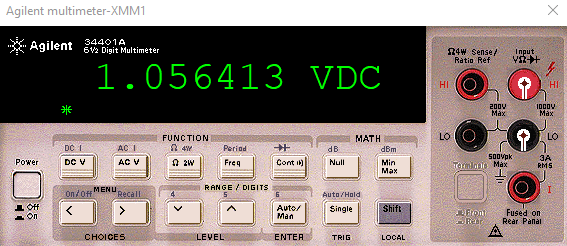
\includegraphics[width=1\textwidth]{1.a.multi.PNG}
    \captionof{figure}{Comprobación del principio de superposición para $\mathbf{R6}$: Voltaje medido en $\mathbf{R6}$ con la fuente de corriente desconectada.}
    \label{fig}
\end{Figura}

\begin{Figura}
    \centering
    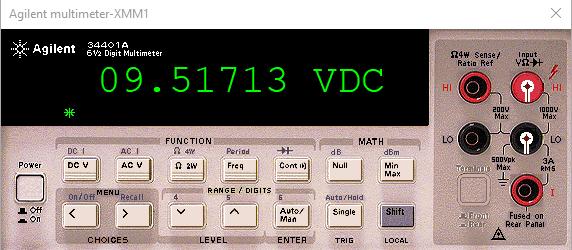
\includegraphics[width=1\textwidth]{1.b.multi.PNG}
    \captionof{figure}{Comprobación del principio de superposición para $\mathbf{R6}$:Voltaje medido en $\mathbf{R6}$ con la fuente de voltaje cortocircuitada y desconectada.}
    \label{fig}
\end{Figura}

\begin{Figura}
    \centering
    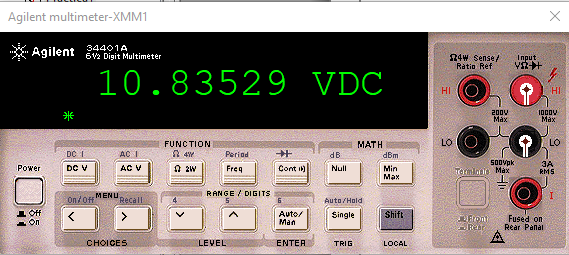
\includegraphics[width=1\textwidth]{1.completo.multi.PNG}
    \captionof{figure}{Comprobación del principio de superposición para $\mathbf{R6}$: Voltaje medido en $\mathbf{R6}$ con el circuito original.}
    \label{fig}
\end{Figura}

\subsubsection*{Objetivo 2}


\begin{Figura}
    \centering
    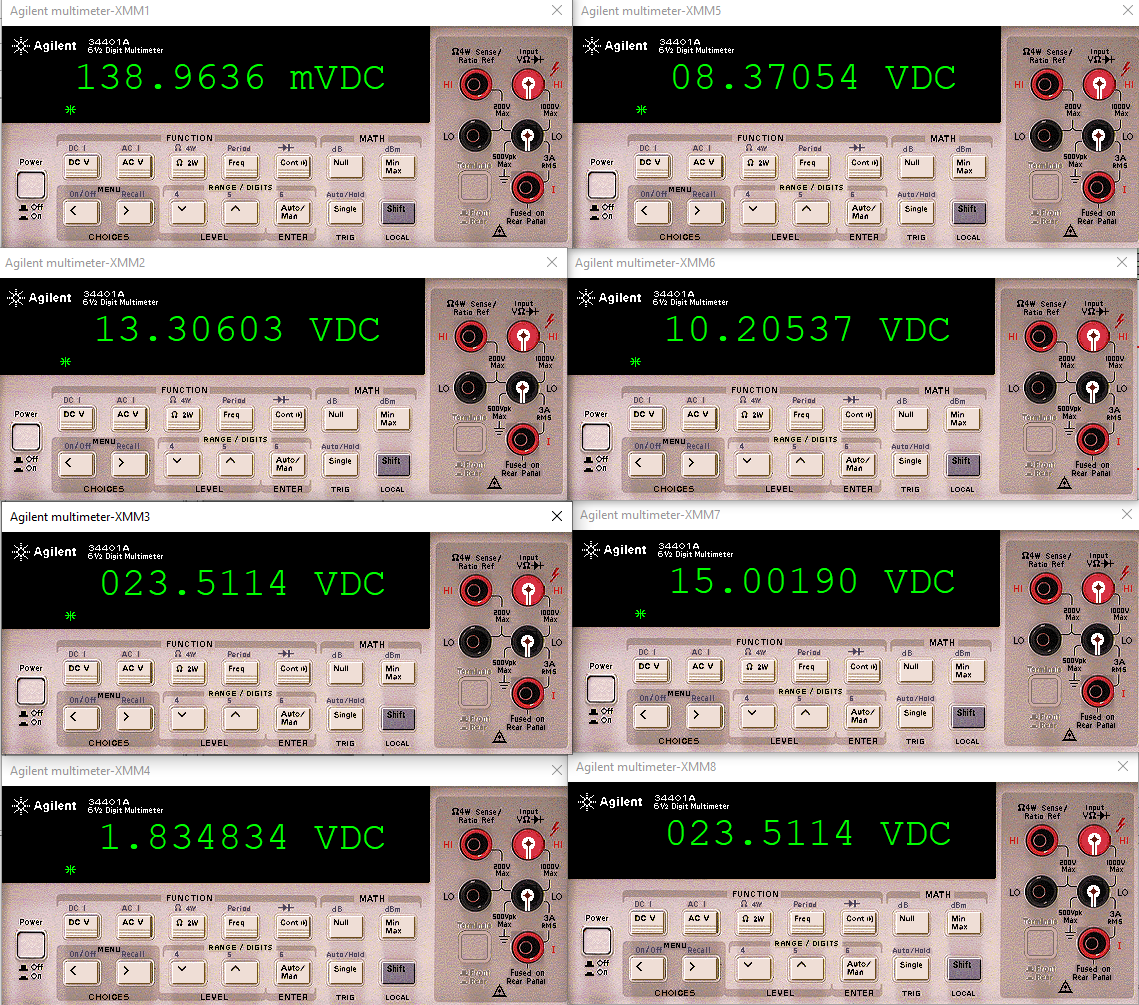
\includegraphics[width=1\textwidth]{voltajes medidos.PNG}
    \captionof{figure}{Medición de voltajes: voltaje medido en cada componente del circuito original.}
    \label{fig}
\end{Figura}

\subsubsection*{Objetivo 3}

\begin{Figura}
    \centering
    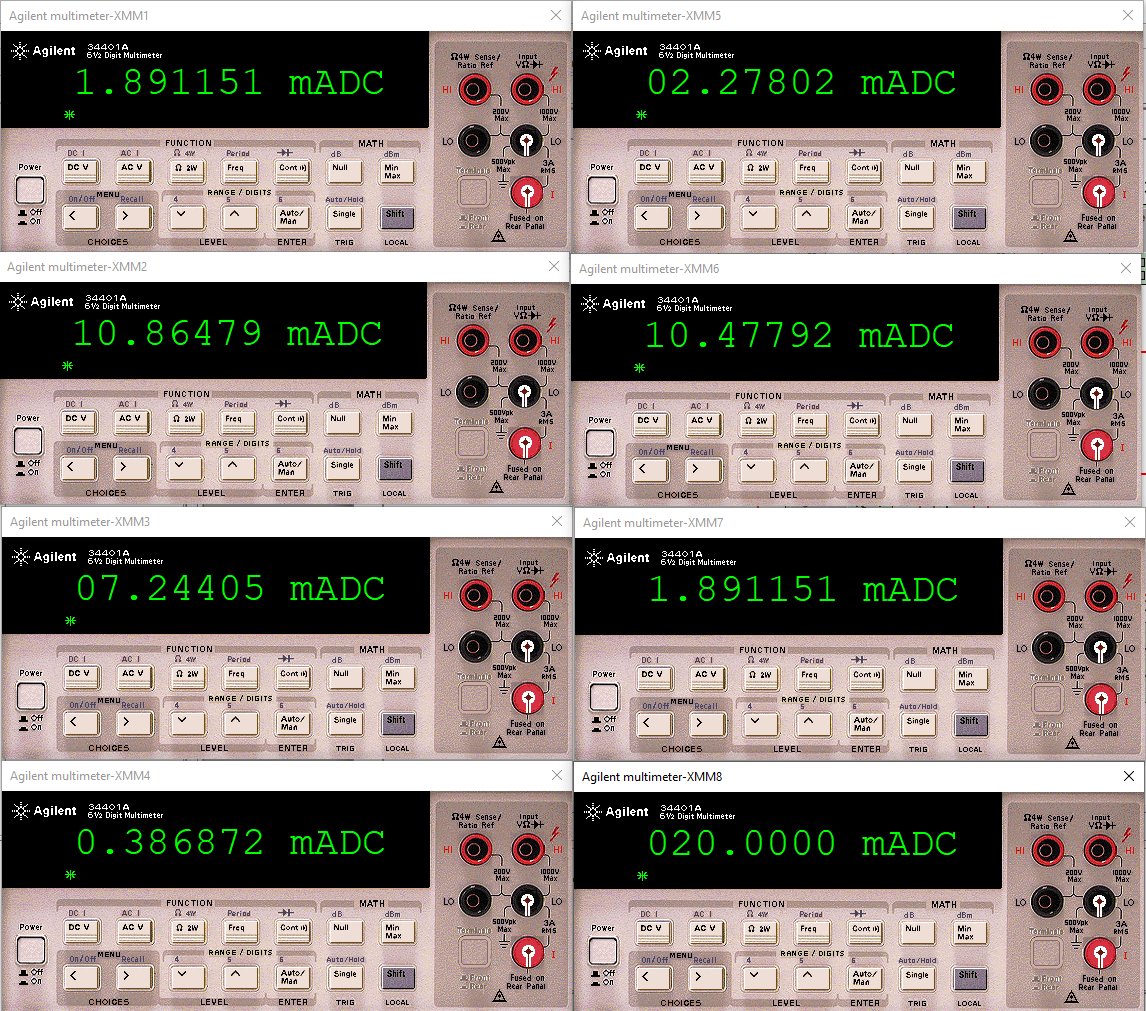
\includegraphics[width=1\textwidth]{corrientes medidas.PNG}
    \captionof{figure}{Medición de corrientes: corriente medida en cada componente del circuito original.}
    \label{fig}
\end{Figura}

\subsubsection*{Objetivo 4}

\begin{Figura}
    \centering
    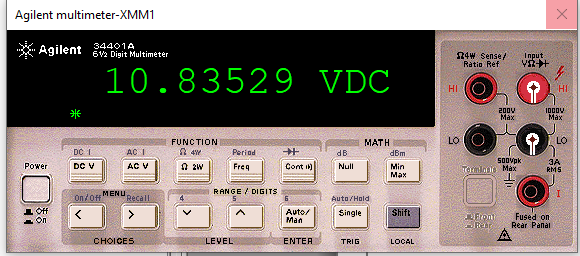
\includegraphics[width=1\textwidth]{T1.multi.PNG}
    \captionof{figure}{Aplicación del teorema de Thévenin en $\mathbf{R6}$: voltaje medido en $\mathbf{R6}$.}
    \label{fig}
\end{Figura}

\begin{Figura}
    \centering
    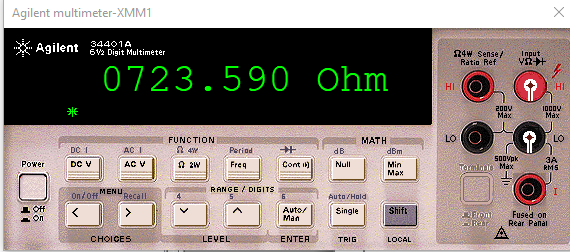
\includegraphics[width=1\textwidth]{T2.multi.PNG}
    \captionof{figure}{Aplicación del teorema de Thévenin en $\mathbf{R6}$: resistencia equivalente medida en $\mathbf{R6}$ con fuente de corriente desconectada y fuente de voltaje cortocitcuitada y desconectada.}
    \label{fig}
\end{Figura}

\subsubsection*{Objetivo 5}

\begin{Figura}
    \centering
    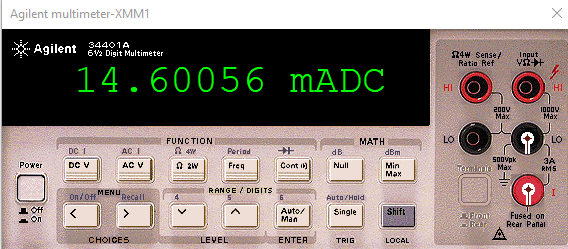
\includegraphics[width=1\textwidth]{N1.multi.PNG}
    \captionof{figure}{Aplicación del teorema de Norton en $\mathbf{R6}$: corriente medida en $\mathbf{R6}$.}
    \label{fig}
\end{Figura}

\begin{Figura}
    \centering
    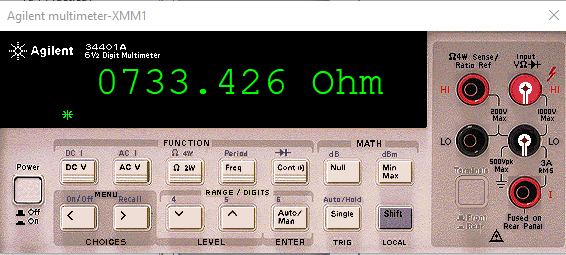
\includegraphics[width=1\textwidth]{N2.multi.PNG}
    \captionof{figure}{Aplicación del teorema de Norton en $\mathbf{R6}$: resistencia equivalente medida en $\mathbf{R6}$ con fuente de corriente desconectada y fuente de voltaje cortocitcuitada y desconectada.}
    \label{fig}
\end{Figura}

\subsection*{Calculo de Incertidumbres}
Para determinar la incertidumbre de cada medición se usa la tabla de incertidumbres presente en el manual del multímetro que también se encuentra en la siguiente subsección.

\subsubsection*{Objetivo 1}



\begin{equation*}
    \delta V_1 = (V_1 \cdot Rd\% + rango(V_1) \cdot Rg\%) 
\end{equation*}

\begin{equation*}
    = (1.056413 \cdot 0.000035 + 10 \cdot 0.000005 ) V = \num{8.697e-7} V
\end{equation*}

\begin{equation*}
    \delta V_2 = (V_2 \cdot Rd\% + rango(V_2) \cdot Rg\%) 
\end{equation*}

\begin{equation*}
    = (9.51713 \cdot 0.000035 + 10 \cdot 0.000005 ) V = \num{3.83e-6} V
\end{equation*}

\begin{equation*}
    \delta V_3 = (V_3 \cdot Rd\% + rango(V_3) \cdot Rg\%) 
\end{equation*}

\begin{equation*}
    = (10.83529 \cdot 0.000045 + 100 \cdot 0.000006 ) V = \num{1.088e-5} V
\end{equation*}

\subsubsection*{Objetivo 2}

\begin{equation*}
    \delta V_1 = (V_1 \cdot Rd\% + rango(V_1) \cdot Rg\%) 
\end{equation*}

\begin{equation*}
    = (138.9636 \cdot 0.000050 + 100 \cdot 0.000035 ) V = 0.0104 mV
\end{equation*}

\begin{equation*}
    \delta V_2 = (V_2 \cdot Rd\% + rango(V_2) \cdot Rg\%) 
\end{equation*}

\begin{equation*}
    = (13.30603 \cdot 0.000035 + 10 \cdot 0.000005 ) V = \num{5.157e-4} V
\end{equation*}

\begin{equation*}
    \delta V_3 = (V_3 \cdot Rd\% + rango(V_3) \cdot Rg\%) 
\end{equation*}

\begin{equation*}
    = (23.514 \cdot 0.000045 + 100 \cdot 0.000006 ) V = \num{1.658e-3} V
\end{equation*}

\begin{equation*}
    \delta V_4 = (V_4 \cdot Rd\% + rango(V_4) \cdot Rg\%) 
\end{equation*}

\begin{equation*}
    = (1.834834 \cdot 0.000035 + 10 \cdot 0.000005 ) V = \num{1.142 e-4} V
\end{equation*}

\begin{equation*}
    \delta V_5 = (V_5 \cdot Rd\% + rango(V_5) \cdot Rg\%) 
\end{equation*}

\begin{equation*}
    = (8.37054 \cdot 0.000035 + 10 \cdot 0.000005 ) V = \num{3.430e-4} V
\end{equation*}

\begin{equation*}
    \delta V_6 = (V_6 \cdot Rd\% + rango(V_6) \cdot Rg\%) 
\end{equation*}

\begin{equation*}
    = (10.20537 \cdot 0.000045 + 100 \cdot 0.000006 ) V = \num{1.059e-3} V
\end{equation*}

\begin{equation*}
    \delta V_7 = (V_7 \cdot Rd\% + rango(V_7) \cdot Rg\%) 
\end{equation*}

\begin{equation*}
    = (15.00190 \cdot 0.000045 + 100 \cdot 0.000006 ) V = \num{1.275e-3} V
\end{equation*}

\begin{equation*}
    \delta V_8 = (V_8 \cdot Rd\% + rango(V_8) \cdot Rg\%) 
\end{equation*}

\begin{equation*}
    = (23.5114 \cdot 0.0045 + 100 \cdot 0.0006 ) V = \num{1.658e-3} V
\end{equation*}

\subsubsection*{Objetivo 3}

\begin{equation*}
    \delta I_1 = (I_1 \cdot Rd\% + rango(I_1) \cdot Rg\%) 
\end{equation*}

\begin{equation*}
    = (1.891151 \cdot 0.00050 + 10 \cdot 0.00020 ) mA = \num{2.946e-3} mA
\end{equation*}

\begin{equation*}
    \delta I_2 = (I_2 \cdot Rd\% + rango(I_2) \cdot Rg\%) 
\end{equation*}

\begin{equation*}
    = (10.86479 \cdot 0.00050 + 100 \cdot 0.00005 ) mA = \num{0.01043} mA
\end{equation*}

\begin{equation*}
    \delta I_3 = (I_3 \cdot Rd\% + rango(I_3) \cdot Rg\%) 
\end{equation*}

\begin{equation*}
    = (7.24405 \cdot 0.00050 + 10 \cdot 0.00020 ) mA = \num{5.622 e-3} mA
\end{equation*}

\begin{equation*}
    \delta I_4 = (I_4 \cdot Rd\% + rango(I_4) \cdot Rg\%) 
\end{equation*}

\begin{equation*}
    = (0.386872 \cdot 0.00050 + 10 \cdot 0.00020 ) mA = \num{2.193 e-3} mA
\end{equation*}

\begin{equation*}
    \delta I_5 = (I_5 \cdot Rd\% + rango(I_5) \cdot Rg\%) 
\end{equation*}

\begin{equation*}
    = (2.27802 \cdot 0.00050 + 10 \cdot 0.00020 ) mA = \num{3.139e-3} mA
\end{equation*}

\begin{equation*}
    \delta I_6 = (I_6 \cdot Rd\% + rango(I_6) \cdot Rg\%) 
\end{equation*}

\begin{equation*}
    = (10.47792 \cdot 0.00050 + 100 \cdot 0.00005 ) mA = 0.01024 mA
\end{equation*}

\begin{equation*}
    \delta I_7 = (I_7 \cdot Rd\% + rango(I_7) \cdot Rg\%) 
\end{equation*}

\begin{equation*}
    = (1.891151 \cdot 0.00050 + 10 \cdot 0.00020 ) mA = \num{2.946 e -3} mA
\end{equation*}

\begin{equation*}
    \delta I_8 = (I_8 \cdot Rd\% + rango(I_8) \cdot Rg\%) 
\end{equation*}

\begin{equation*}
    = (20 \cdot 0.00050 + 100 \cdot 0.00005 ) mA = \num{0.015} mA
\end{equation*}



\subsubsection*{Objetivo 4}

\begin{equation*}
    \delta V = (V \cdot Rd\% + rango(V) \cdot Rg\%) 
\end{equation*}

\begin{equation*}
    = (10.83529 \cdot 0.000045 + 100 \cdot 0.000006 ) V = \num{1.0888e-3} V
\end{equation*}

\begin{equation*}
    \delta R = (R \cdot Rd\% + rango(R) \cdot Rg\%) 
\end{equation*}

\begin{equation*}
    = (723.590 \cdot 0.00010 + 1000 \cdot 0.00001 ) \Omega = 0.082 \Omega
\end{equation*}





\subsubsection*{Objetivo 5}

\begin{equation*}
    \delta I = (I \cdot Rd\% + rango(I) \cdot Rg\%) 
\end{equation*}

\begin{equation*}
    = (14.60056 \cdot 0.00050 + 100 \cdot 0.00005 ) mA = 0.01230 mA
\end{equation*}

\begin{equation*}
    \delta R = (R \cdot Rd\% + rango(R) \cdot Rg\%) 
\end{equation*}

\begin{equation*}
    = (723.426 \cdot 0.00010 + 1000 \cdot 0.00001 ) \Omega = 0.082 \Omega
\end{equation*}





\end{multicols}



\subsection*{Incertidumbres para el multímetro}

\begin{Figura}
    \centering
    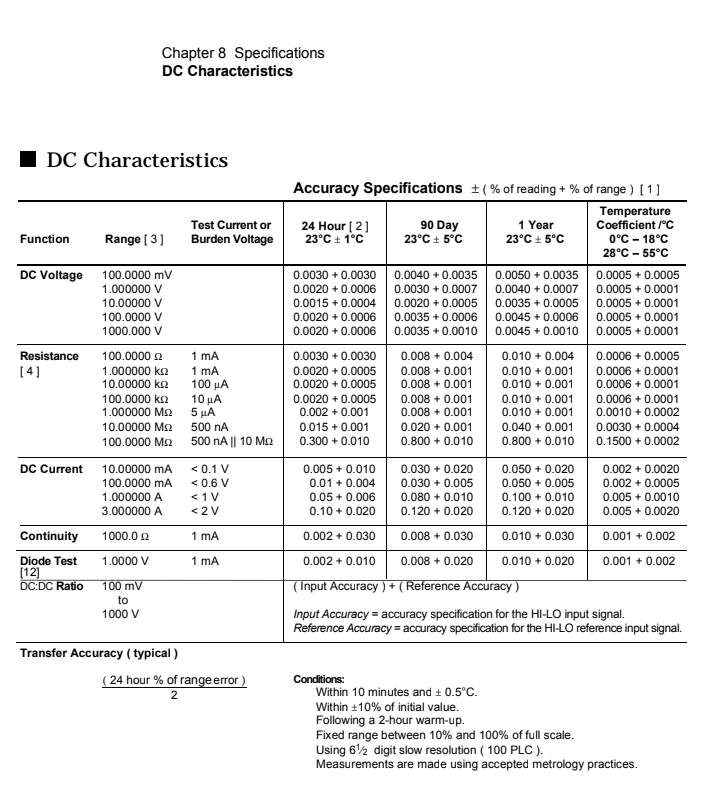
\includegraphics[width=1\textwidth]{incertidumbres multimetro.PNG}
    \captionof{figure}{Tabla de incertidumbres para el multímetro Aligent 34401A}
    \label{fig}
\end{Figura}





\end{document}